% Source: graduate-coursework/Research/Intro_to_Agents/handouts/Part3_Basic_Usage.tex

\documentclass[border=4pt]{standalone}
\usepackage[T1]{fontenc}
\usepackage{graphicx}
\usepackage{lmodern}
\usepackage{tikz}
\usepackage{xcolor}
\usetikzlibrary{shapes.geometric,arrows.meta,positioning,calc,fit,backgrounds,decorations.pathreplacing}

\definecolor{UofSCGarnet}{HTML}{73000a}
\definecolor{UofSCBlack}{HTML}{000000}
\definecolor{UofSCWhite}{HTML}{ffffff}
\definecolor{UofSCRose}{HTML}{CC2E40}
\definecolor{UofSCAtlantic}{HTML}{466A9F}
\definecolor{UofSCCongaree}{HTML}{1F414D}
\definecolor{UofSCHorseshoe}{HTML}{65780B}
\definecolor{UofSCGrass}{HTML}{CED318}
\definecolor{UofSCHoneycomb}{HTML}{A49137}
\definecolor{UofSC90Black}{HTML}{363636}
\definecolor{UofSC70Black}{HTML}{5C5C5C}
\definecolor{UofSC50Black}{HTML}{A2A2A2}
\definecolor{UofSCWarmGrey}{HTML}{676156}
\definecolor{UofSCSandstorm}{HTML}{FFF2E3}
\definecolor{UofSCDarkGarnet}{HTML}{570008}
\definecolor{UofSCAzalea}{HTML}{844247}

\tikzset{
    % Sharp-cornered boxes
    process/.style={
        rectangle,
        draw=UofSCBlack,
        thick,
        fill=UofSCWhite,
        text=UofSCBlack,
        minimum width=3cm,
        minimum height=0.8cm,
        align=center,
        font=\small
    },
    process highlight/.style={
        process,
        fill=UofSCGarnet,
        text=UofSCWhite
    },
    process secondary/.style={
        process,
        fill=UofSCAtlantic,
        text=UofSCWhite
    },
    process tertiary/.style={
        process,
        fill=UofSCCongaree,
        text=UofSCWhite
    },
    arrow/.style={
        ->,
        >=Stealth,
        thick,
        color=UofSCBlack
    },
    arrow garnet/.style={
        arrow,
        color=UofSCGarnet
    },
    label box/.style={
        rectangle,
        draw=none,
        fill=UofSCSandstorm,
        text=UofSCBlack,
        font=\scriptsize,
        align=center
    },
    decision/.style={
        diamond,
        draw=UofSCBlack,
        thick,
        fill=UofSCHoneycomb,
        text=UofSCBlack,
        minimum width=2cm,
        minimum height=1cm,
        align=center,
        font=\small,
        aspect=2
    }
}

\begin{document}
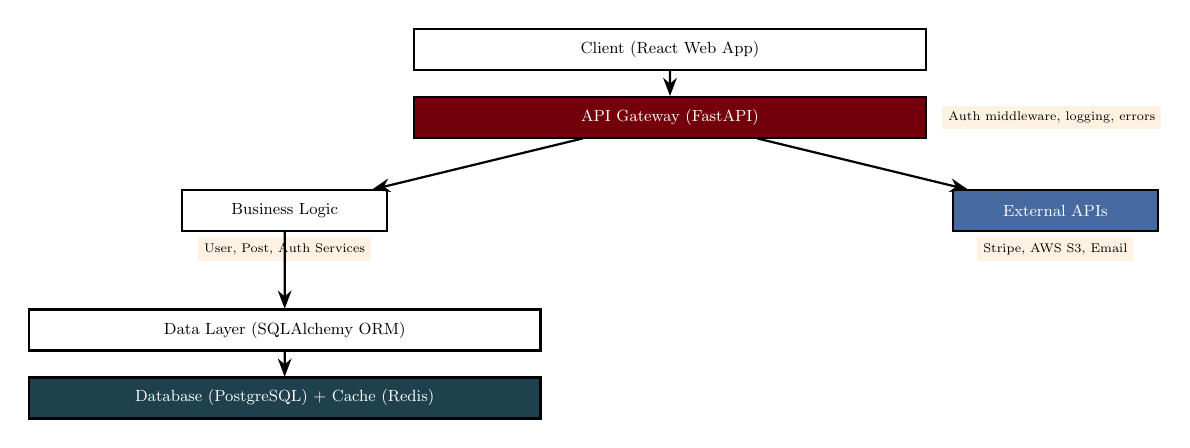
\begin{tikzpicture}[node distance=0.5cm, scale=0.65, transform shape]
        % Client layer
        \node[process, minimum width=10cm] (client) {Client (React Web App)};

        % API Gateway
        \node[process highlight, below=of client, minimum width=10cm] (api) {API Gateway (FastAPI)};
        \node[label box, right=0.3cm of api] {\scriptsize Auth middleware, logging, errors};

        % Services layer
        \node[process, below left=1cm and 0.5cm of api, minimum width=4cm] (business) {Business Logic};
        \node[process secondary, below right=1cm and 0.5cm of api, minimum width=4cm] (external) {External APIs};

        \node[label box, below=0.1cm of business] {\scriptsize User, Post, Auth Services};
        \node[label box, below=0.1cm of external] {\scriptsize Stripe, AWS S3, Email};

        % Data layer
        \node[process, below=1.5cm of business, minimum width=10cm] (data) {Data Layer (SQLAlchemy ORM)};

        % Database
        \node[process tertiary, below=of data, minimum width=10cm] (db) {Database (PostgreSQL) + Cache (Redis)};

        % Arrows
        \draw[arrow] (client) -- (api);
        \draw[arrow] (api) -- (business);
        \draw[arrow] (api) -- (external);
        \draw[arrow] (business) -- (data);
        \draw[arrow] (data) -- (db);
    \end{tikzpicture}
\end{document}
